%\documentclass[12pt]{article}
\documentclass[12pt, a4paper, openright, twoside]{report}
\usepackage{emptypage}
\pagenumbering{gobble}
\usepackage{natbib}
\usepackage{makecell}
%\usepackage{geometry}

\usepackage{booktabs}


\usepackage{pdfpages}
\usepackage{lscape}
\usepackage{hyperref}

\hypersetup{
    colorlinks=true,
    linkcolor=black,
    %filecolor=magenta,
    urlcolor=black,
    breaklinks=false,
   citecolor=black,
}
\usepackage[nottoc,notlof,notlot]{tocbibind}
\usepackage{framed}
%\usepackage{svg}
%\usepackage{amsmath}
\usepackage{rotfloat}
\usepackage{subfig}
\usepackage{graphicx}
\usepackage{caption}
\captionsetup[table]{skip=10pt}
\usepackage{graphicx}
\usepackage[utf8]{inputenc}
%\usepackage[center]{titlesec}
\usepackage{verbatim}
\usepackage[utf8]{inputenc}
\usepackage{amsmath}
\usepackage{algorithm2e,setspace}
\usepackage{algorithm}
\usepackage{algorithmic}
\usepackage[english]{babel}
%\usepackage[ruled,vlined]{algorithm2e}
%\usepackage[noend]{algpseudocode}
%\usepackage{array}
\usepackage{float}
\usepackage{tikz}
\usepackage{pgfplots}
\usepackage{pbox}
\usepackage{url}
\usepackage{tkz-graph}
%\usepackage{graphicx,subfigure}
%\usepackage{vaucanson-g}
\usepackage{array}
\usepackage{amssymb}
\usepackage{fancyvrb}
\usepackage{listings}
\usepackage{ragged2e}
\usepackage{slashbox}
\makeatletter
\def\BState{\State\hskip-\ALG@thistlm}
\makeatother
\usepackage{sectsty}
\usepackage{comment}
\usepackage{soul}
\usepackage{array}
\usepackage{chngcntr}
\usepackage{cancel}
\usepackage{multirow}
%\usepackage{subfigure}
\usepackage[toc,page]{appendix}
\usepackage{tikz}
\usepackage{setspace}
\usepackage{afterpage}
\usetikzlibrary{shapes,arrows,positioning,calc}
\graphicspath{ {images/} }
%\topmargin -23 mm
\providecommand{\keywords}[1]{\textbf{\textit{Keywords---}} #1}
%\headheight 8pt
%\oddsidemargin 0mm
%\evensidemargin -5mm
\textwidth 161mm
\textheight 210mm
\linespread{1}
%\footskip = 60pt
\usepackage{titlesec}
\chapterfont{\centering}
\newcolumntype{P}[1]{>{\centering\arraybackslash}p{#1}}
\newcolumntype{M}[1]{>{\centering\arraybackslash}m{#1}}
%\geometry{a4paper, portrait, margin=1in}
\renewcommand{\baselinestretch}{1.3}
\titleformat{\chapter}[display]
{\normalfont\huge\bfseries\centering}{\chaptertitlename\ \thechapter}{10pt}{\Huge\centering}
\titlespacing*{\chapter}{0pt}{-50pt}{5pt}
\usepackage{pdfpages}

\usepackage[
 top    = 1.5in,
  bottom = 1in,
  left   = 1.5in,
  right  = 1in,
  %headsep=5mm,%%% Example
  %includeheadfoot%%%%%%%%%%%%%%%%%%%%%%%%%%
  ]{geometry}
%below code used for page bordering
\iffalse
\usepackage{pgf}
\usepackage{pgfpages}
%
\pgfpagesdeclarelayout{boxed}
{
  \edef\pgfpageoptionborder{4pt}
}
{
  \pgfpagesphysicalpageoptions
  {%
    logical pages=1,%
  }
  \pgfpageslogicalpageoptions{1}
  {
    border code=\pgfsetlinewidth{1.5pt}\pgfstroke,%
    border shrink=\pgfpageoptionborder,%
    resized width=.95\pgfphysicalwidth,%
    resized height=.95\pgfphysicalheight,%
    center=\pgfpoint{.5\pgfphysicalwidth}{.5\pgfphysicalheight}%
  }%
}
\pgfpagesuselayout{boxed}
\setlength{\parindent}{2cm}
\usetikzlibrary{calc}
\usepackage{eso-pic}
\fi
\begin{document}
\counterwithin{table}{chapter}
\counterwithin{figure}{chapter}
\thispagestyle{empty}
%\begin{titlepage}
\iffalse
\AddToShipoutPictureBG*{%
\begin{tikzpicture}[overlay,remember picture]
\draw[line width=4pt]
    ($ (current page.north west) + (1cm,-1cm) $)
    rectangle
    ($ (current page.south east) + (-1cm,1cm) $);
\draw[line width=1.5pt]
    ($ (current page.north west) + (1.2cm,-1.2cm) $)
    rectangle
    ($ (current page.south east) + (-1.2cm,1.2cm) $);
\end{tikzpicture}
}
\fi



\begin{center}
Major Project-I Report on \\
  % \textbf{Major Project-I Report on} \\
 \null
 \textbf{\large GMVD: Smart Contract Vulnerability Detection Based on GAT-Mamba Framework}\\
 \null
\null
% Thesis\\
Submitted in partial fulfillment of the requirements for the degree of\\
 \null
 MASTER OF TECHNOLOGY\\
in\\
INFORMATION TECHNOLOGY\\
 \null


by \\
\large{\textbf{AMEESHA PATEL}} \\
{\textbf{(252IT003)}}\\
%\textbf{M.Tech. (IT)}\\
\vspace{2em}
		\large{\textit{under the guidance of}} \\
		\vspace{0.2em}

		\large{\textbf{Dr. JANANI T.}}\\
		\vspace{1em}
\begin{figure}[h] % b - bottom, t - top, h - here
 \centering{

\includegraphics[width=4cm, height=4cm]{NITKLogo.jpeg}
 }
\end{figure}

DEPARTMENT OF INFORMATION TECHNOLOGY\\
NATIONAL INSTITUTE OF TECHNOLOGY KARNATAKA\\
SURATHKAL, MANGALORE - 575025

August, 2026\\
\end{center}

\clearpage
\newpage

\ % The empty page

\newpage
\thispagestyle{empty}

\begin{framed}
\begin{center}
\textbf{{\Large DECLARATION}}\\
\end{center}
\null
I hereby \textit{declare} that the Report of the P.G. Major Project-I Work entitled ``GMVD: Smart Contract Vulnerability Detection Based on GAT-Mamba Framework'', which is being submitted to National Institute of Technology Karnataka, Surathkal, in partial fulfillment of the requirements for the award of the Degree of Master of Technology in Information Technology in the Department of Information Technology, is a \textit{bonafide report of the work carried out by me.} The material contained in this report has not been submitted at any University or Institution for the award of any degree.\\
\\
\\
\\
\\
\null \hfill AMEESHA PATEL (252IT003)\\
\null \hfill Dept. of Information Technology\\
\null \hfill NITK Surathkal, Mangalore\\
\\
Place: NITK, Surathkal
\\
Date: 31 August, 2026
\end{framed}
\clearpage
\newpage

\ % The empty page

\newpage

\begin{framed}
\begin{center}
\textbf{{\Large CERTIFICATE}} \\
\end{center}
\null
This is to \textit{certify} that the P.G Major Project-I Work entitled ``GMVD: Smart Contract Vulnerability Detection Based on GAT-Mamba Framework'',
submitted by AMEESHA PATEL (252IT003) as the record of the work carried out by her, is \textit{accepted as the P.G. Project Work report submission} in partial fulfillment of the requirement for the award of degree of Master of Technology in Information Technology in the Department of Information Technology, NITK Surathkal, India.
\\
\\
\\
\\
\\
\\

\begin{center}
    Dr. JANANI T.\\

    (Signature of the guide with Date and Seal)\\
%NITK Surathkal, Mangalore\hfill NITK Surathkal, Mangalore
\null
\null
\null
\null
\null

    Chairman - DPGC\\
    (Signature with Date and Seal)
\end{center}
\end{framed}

\thispagestyle{empty}


\clearpage
\newpage

\ % The empty page

\newpage
\thispagestyle{empty}
\begin{center}
\textbf{{\Large ACKNOWLEDGEMENT}}\\
\end{center}
\null
I would sincerely like to thank Dr. Janani T. for her unconditional and unbiased support during the whole session of study and development, and for guiding me throughout the course of this Minor Project. Her valuable feedback on the choice of architecture, the experimental design, and the interpretation of results was instrumental in shaping this work. I would also like to thank the Department of Information Technology, NITK Surathkal, for providing the resources and environment necessary to carry out this project.
\\
\\
\null \hfill AMEESHA PATEL
\\
\clearpage
\cleardoublepage

\begin{center}
%\chapter*{Abstract}
\textbf{{\Large ABSTRACT}}\\
\end{center}

Smart contracts are self-executing programs deployed on blockchain platforms such as Ethereum, and their immutability and direct control over digital assets make security vulnerabilities in their code particularly costly. Reentrancy, block-timestamp dependence, and infinite-loop vulnerabilities are among the most frequently exploited classes of defects in deployed Solidity contracts, and manual auditing and traditional static-analysis tools do not scale well to the volume of contracts deployed today.

This project implements and evaluates GMVD, a deep-learning framework for function-level smart contract vulnerability detection that combines four components: a set of hand-designed local expert patterns capturing known vulnerability idioms, a Graph Attention Network (GAT) that encodes a function's control-flow/data-flow semantic graph into a graph-level feature vector, a Mamba-style selective state-space (S6) block that fuses the local patterns and the graph feature into an updated feature sequence, and a cross-attention fusion layer with a multi-layer perceptron (MLP) classifier that produces the final vulnerability prediction along with an interpretable per-feature attention weight.

The framework is implemented end-to-end in PyTorch and trained from scratch on labeled datasets for three vulnerability types -- reentrancy, timestamp dependence, and infinite loop -- covering thousands of real, previously audited Solidity functions. In addition to the full GMVD model, three ablated variants (removing the GAT, the Mamba block, or both) and five baseline models (a graph-only GCN, three sequence baselines over the local patterns, and an attention-gated reimplementation of an expert-pattern baseline) are trained and evaluated under an identical experimental protocol, giving a total of nine models evaluated per vulnerability type.

The trained models are evaluated using accuracy, precision, recall, F1-score, and ROC-AUC, and the resulting confusion matrices, ROC curves, and per-feature interpretability weights are analysed to understand both the predictive performance and the relative contribution of local expert patterns versus the global graph feature for each vulnerability type. The project demonstrates a complete, reproducible pipeline for building and evaluating an interpretable, graph- and state-space-based smart contract vulnerability detector.

\hspace{1cm}
\null
\\
\\
\keywords{Smart Contract Security, Vulnerability Detection, Graph Attention Network, Mamba, State-Space Model, Cross-Attention, Reentrancy, Timestamp Dependence, Infinite Loop.}

\renewcommand*{\contentsname}{\MakeUppercase{Contents}}
\renewcommand*{\listfigurename}{\MakeUppercase{List of Figures}}
\renewcommand*{\listtablename}{\MakeUppercase{List of Tables}}
\renewcommand{\bibname}{REFERENCES}
\thispagestyle{}
\pagenumbering{roman}
\setcounter{page}{1}
\clearpage
\addtocontents{toc}{\protect\thispagestyle{}}
\tableofcontents
\clearpage
\addcontentsline{toc}{chapter}{LIST OF FIGURES}
\listoffigures
\clearpage
\begingroup
\let\clearpage\relax
\null
\null
\null
\addcontentsline{toc}{chapter}{LIST OF TABLES}
\listoftables
\endgroup
\cleardoublepage
\newgeometry{top    = 1in,
  bottom = 1in,
  left   = 1.65in,
  right  = 1in, }
% \begin{center}
\begin{center}

\textbf{{\huge ABBREVIATIONS}}
\addcontentsline{toc}{chapter}{ABBREVIATIONS}

\input{acro.txt}
\end{center}
\null
\restoregeometry

\cleardoublepage
\newgeometry{top    = 1.5in,
  bottom = 1in,
  left   = 1.65in,
  right  = 1in, }
% \textbf{{\huge ABBREVIATIONS}}
% \addcontentsline{toc}{chapter}{ABBREVIATIONS}

% \end{center}
% \null
% \restoregeometry

% \cleardoublepage
% \newgeometry{top    = 1.5in,
%   bottom = 1in,
%   left   = 1.65in,
%   right  = 1in, }
\chapter{Introduction}

\pagenumbering{arabic}
\setcounter{page}{1}

\section{Background}

Blockchain platforms such as Ethereum allow developers to deploy self-executing programs, known as smart contracts, that manage digital assets and enforce agreements without a trusted intermediary. Once deployed, a smart contract's bytecode is immutable and its execution is transparent and irreversible, which means that any security flaw present at deployment time remains permanently exploitable unless the contract is explicitly designed to be upgradeable. Because smart contracts frequently hold or control significant amounts of cryptocurrency and other digital assets, vulnerabilities in their code have repeatedly led to large financial losses.

Among the many classes of smart contract vulnerabilities, three are particularly common and well studied: \textit{reentrancy}, in which an external call within a function allows a malicious contract to recursively re-enter the calling function before its state has been fully updated; \textit{timestamp dependence}, in which contract logic relies on the block timestamp (\texttt{block.timestamp}) as a source of randomness or as a critical decision variable, even though miners have some latitude to manipulate this value; and \textit{infinite loop}, in which unbounded or unexpectedly long loops cause a transaction to exhaust its gas allowance, resulting in a denial of service for the function.

Traditional approaches to detecting these vulnerabilities rely on static analysis, symbolic execution, or manually written pattern-matching rules, implemented in tools such as Oyente, Mythril, Securify, Slither, and Smartcheck. While useful, these tools require vulnerability patterns to be manually encoded in advance, can produce a large number of false positives, and typically analyze each contract independently of the vast body of previously audited contracts. This has motivated a growing body of work that applies machine learning, and in particular deep learning on graph-structured and sequential representations of contract code, to automatically learn what a vulnerable function looks like from labeled examples.

\section{Motivation}

A central design tension in learning-based vulnerability detection is the choice of representation. Graph-based models (such as graph convolutional or graph attention networks) naturally capture the control-flow and data-flow structure of a function, but on their own may not exploit the domain knowledge already encoded in hand-designed expert patterns for a specific vulnerability type. Conversely, models that rely purely on expert patterns do not benefit from the broader structural context of the function. Prior work such as AME (Attention-based Model with Expert patterns) addressed this by fusing a graph feature with expert patterns through a learned attention mechanism, and demonstrated that combining both sources of information, together with an interpretable attention weight, improves detection performance and gives auditors insight into which signal (structure or pattern) drove a given prediction.

The GMVD framework studied in this project extends this line of work along two axes. First, it replaces the graph encoder with a Graph Attention Network, allowing the model to learn which neighboring statements are most relevant to a given node rather than aggregating neighbors uniformly. Second, it introduces a Mamba-style selective state-space block to fuse the local expert patterns and the global graph feature before the final cross-attention and classification stage, in place of a plain concatenation or single attention layer. State-space sequence models of this kind process a sequence with linear-time recurrence and an input-dependent (selective) state update, which allows the model to propagate and gate information between the pattern and graph features in a data-dependent way. Combining GAT-based structural encoding with an S6-based fusion stage, followed by cross-attention and an interpretable classification head, is the central idea evaluated in this project.

\section{Organisation of the Report}

The remainder of this report is organized into five chapters.

Chapter 2 presents the literature review covering static-analysis tools for smart contracts, graph neural network based vulnerability detectors, expert-pattern and attention-based fusion models, and state-space sequence models, followed by the outcome of the review, the problem statement, and the objectives of this project.

Chapter 3 describes the proposed methodology, including the vulnerability types considered, the graph and local-pattern representation of a function, the GAT encoder, the Mamba/S6 fusion block, the cross-attention classification head, the ablation and baseline models, the training procedure, and the evaluation metrics.

Chapter 4 describes the work done, including the experimental setup (software environment, datasets, preprocessing, and hyperparameters) and the experimental results (dataset statistics, the full comparison across all trained models, the ablation study, confusion matrices, ROC curves, interpretability analysis, and computational cost).

Chapter 5 concludes the project and discusses its limitations and directions for future work.

\chapter{Literature Review}
\label{literaturereview}
\vspace{3em}

Early tools for smart contract security analysis, including Oyente, Mythril, Securify, Slither, and Smartcheck, rely on symbolic execution or static pattern matching against a fixed catalogue of vulnerability signatures. These tools do not require labeled training data and can provide precise traces for the vulnerabilities they are designed to detect, but their coverage is limited to patterns their authors anticipated, and they analyze each contract in isolation without learning from a corpus of previously labeled examples.

Graph neural network (GNN) based approaches recast a smart contract function as a graph -- typically built from its control-flow and data-flow structure -- and train a classifier on labeled examples to learn which structural patterns correlate with a vulnerability. Zhuang \textit{et al.} proposed a degree-aware graph convolutional baseline together with a Temporal Message Propagation network (TMP) that explicitly models the temporal order of statements along the control-flow graph, and showed that graph-based learning outperforms purely sequence-based deep learning models for reentrancy and timestamp-dependence detection.

Building on this, Liu \textit{et al.} proposed AME, which represents a function using both a graph feature (produced by a graph encoder) and three hand-designed local expert patterns capturing vulnerability-specific code idioms, and fuses the two using a learned attention mechanism. AME additionally exposes an interpretable weight for each of the four features (the three local patterns and the graph feature), allowing an auditor to see which signal contributed most to a given prediction. This expert-pattern-plus-attention design forms the direct basis for the GMVD framework studied in this project.

Graph Attention Networks (GAT), introduced by Velickovic \textit{et al.}, generalize graph convolution by learning an attention coefficient for each edge rather than using a fixed or degree-normalized aggregation weight, allowing the encoder to focus on the most relevant neighboring nodes for a given node's representation. This makes GAT a natural replacement for the plain graph convolutional encoders used in earlier smart-contract vulnerability detectors.

Separately, Mamba, introduced by Gu and Dao, is a selective state-space sequence model (S6) that processes a sequence with an input-dependent (selective) recurrence, achieving linear-time complexity in sequence length while retaining the ability to selectively propagate or discard information at each step. Although originally proposed for long-sequence modeling tasks such as language modeling, its selective gating mechanism is also well suited to fusing a small number of heterogeneous feature vectors -- such as the local expert patterns and the graph feature used in this project -- before a final classification stage.

The GMVD framework combines these three lines of work: a GAT-based graph encoder in place of a plain GCN, a Mamba/S6 block for fusing the local expert patterns with the graph feature, and a cross-attention layer with an interpretable classification head in the style of AME.

\begin{table}[h!]
\centering
\caption{Summary of literature survey for the most relevant related works}
\begin{tabular}{|p{3.6cm}|p{6cm}|p{4.5cm}|}
\hline
\textbf{Authors} & \textbf{Methodology} & \textbf{Observation} \\
\hline
Zhuang \textit{et al.} (IJCAI 2020) & Degree-aware GCN and Temporal Message Propagation network (TMP) over control-flow graphs & Graph-based models outperform sequence-only deep learning for reentrancy/timestamp detection \\
\hline
Liu \textit{et al.} (IJCAI 2021), AME & Graph feature fused with 3 local expert patterns via learned attention & Interpretable per-feature weights; fusion outperforms either signal alone \\
\hline
Velickovic \textit{et al.} (ICLR 2018), GAT & Attention-weighted neighbour aggregation in a GNN & Learned attention over edges improves on fixed/degree-normalized aggregation \\
\hline
Gu and Dao (2023), Mamba & Selective state-space (S6) sequence model with linear-time recurrence & Input-dependent gating enables selective propagation of information along a sequence \\
\hline
\end{tabular}
\label{littab}
\end{table}

\section{Outcome of Literature Review}
The literature survey indicates that combining structural (graph-based) information with hand-designed local expert patterns, and exposing an interpretable attention weight over both, is an effective strategy for smart contract vulnerability detection. It further suggests that the two components of this combination -- the graph encoder and the fusion mechanism -- can each be improved independently: the graph encoder by adopting attention-based aggregation (GAT), and the fusion mechanism by adopting a selective state-space model (Mamba/S6) in place of a single attention layer. This motivates evaluating a framework, GMVD, that incorporates both improvements together with a final cross-attention classification head, and comparing it against graph-only, pattern-only, and simpler fusion baselines.


\section{Problem Statement}
To develop a learned model that predicts, at function granularity, whether a Solidity smart contract function is vulnerable to reentrancy, timestamp dependence, or infinite loops, while producing an interpretable breakdown of its reliance on local expert patterns versus the global graph structure.


\section{Objectives}

\begin{enumerate}
    \item To implement the local expert pattern extraction, semantic graph construction, GAT graph encoder, Mamba/S6 fusion block, and cross-attention classification head that make up the GMVD framework.

    \item To train and evaluate GMVD on labeled datasets for three vulnerability types: reentrancy, timestamp dependence, and infinite loop.

    \item To implement three ablated variants of GMVD (removing the GAT encoder, the Mamba block, or both) to study the contribution of each architectural component.

    \item To implement five baseline models -- a graph-only GCN, three sequence baselines (Vanilla-RNN, LSTM, GRU) over the local expert patterns, and an attention-gated expert-pattern model (AME-lite) -- for comparison against GMVD.

    \item To evaluate all models using accuracy, precision, recall, F1-score, and ROC-AUC, and to analyze confusion matrices and ROC curves for the full GMVD model.

    \item To compute and analyze the interpretability weights produced by GMVD, showing the relative contribution of each local pattern and the global graph feature to the final prediction for each vulnerability type.

\end{enumerate}

\section{Summary}
This chapter reviewed the progression of smart contract vulnerability detection from static-analysis tools, through graph neural network based classifiers, to attention-based fusion of graph features with expert patterns, and introduced Graph Attention Networks and the Mamba selective state-space model as the two architectural components combined in GMVD. Based on this review, a problem statement and a set of concrete objectives were formulated for implementing and evaluating the GMVD framework. The next chapter presents the detailed methodology followed in this project.

\chapter{Methodology}
\label{methodology}

GMVD predicts, for a single smart-contract function, whether it contains a given vulnerability, using four stages: (1) local expert pattern extraction, (2) semantic graph construction and GAT-based graph feature extraction, (3) Mamba/S6-based fusion of the local patterns and the graph feature, and (4) cross-attention fusion followed by an MLP classifier that produces both the final prediction and an interpretable per-feature weight. A separate model is trained independently for each of the three vulnerability types (reentrancy, timestamp dependence, infinite loop), since each vulnerability is associated with its own set of local expert patterns and its own labeled dataset.

The overall methodology is divided into the following stages:

\begin{enumerate}
    \item Construction of a semantic graph for each labeled function and extraction of its local expert patterns.
    \item Normalization of the semantic graph to a fixed set of core nodes with associated feature vectors and edges.
    \item Encoding of the core-node graph using a Graph Attention Network to obtain a graph-level feature vector.
    \item Projection of the local expert patterns and the graph feature into a shared embedding space.
    \item Fusion of the pattern and graph features, stacked as a four-element sequence, using a Mamba/S6 selective state-space block.
    \item Cross-attention fusion of the resulting sequence, followed by an MLP and a linear classification head.
    \item Computation of an interpretable attention weight for each of the four fused features.
    \item Training with a class-weighted binary cross-entropy loss and early stopping on validation F1-score.
    \item Evaluation using accuracy, precision, recall, F1-score, and ROC-AUC.
\end{enumerate}

\section{Vulnerability Types Considered}

Three function-level vulnerability types are considered, each treated as an independent binary classification problem:

\begin{itemize}
    \item \textbf{Reentrancy:} a function makes an external call (e.g. \texttt{call.value()}) before updating its own state variables, allowing a malicious callee to recursively re-enter the function and repeat an action (such as a withdrawal) before the original state update takes effect.
    \item \textbf{Timestamp dependence:} a function's control flow or a critical computation depends on \texttt{block.timestamp}, which can be influenced within a limited range by the block-producing miner, making the function's behaviour manipulable.
    \item \textbf{Infinite loop:} a function contains a loop whose termination condition can fail to be satisfied for certain inputs or contract states, causing the transaction to run out of gas and revert, denying service to legitimate callers.
\end{itemize}

\section{System Architecture}

Figure~\ref{fig:architecture} shows the overall architecture of GMVD. A function is represented in two complementary ways: as a set of three local expert patterns $P_1, P_2, P_3$, each a fixed-size embedding capturing a hand-designed vulnerability-specific code idiom, and as a semantic graph over the function's core nodes, which is encoded by a GAT into a single graph-level feature vector $g$. The four features $[P_1, P_2, P_3, g]$ are stacked into a sequence, refined by a Mamba/S6 block, and then fused by a cross-attention layer whose output is passed through an MLP and a linear classifier to produce the final prediction, together with an interpretability weight for each of the four features.

\begin{figure}[H]
  \centering
\resizebox{0.92\linewidth}{!}{
\begin{tikzpicture}[
    node distance=0.9cm,
    box/.style={rectangle, draw, rounded corners, align=center, minimum width=4.6cm, minimum height=0.9cm, font=\small},
    smallbox/.style={rectangle, draw, rounded corners, align=center, minimum width=3.6cm, minimum height=0.8cm, font=\small},
    arrow/.style={->, thick}
]

\node[box] (input) {Smart Contract Function};
\node[smallbox, below left=0.9cm and -0.3cm of input] (patterns) {Local Expert Pattern\\Extraction ($P_1,P_2,P_3$)};
\node[smallbox, below right=0.9cm and -0.3cm of input] (graph) {Semantic Graph\\Construction + GAT ($g$)};
\node[box, below=1.6cm of input] (stack) {Stack as Sequence $[P_1,P_2,P_3,g]$};
\node[box, below=of stack] (mamba) {Mamba / S6 Selective\\State-Space Fusion};
\node[box, below=of mamba] (crossattn) {Cross-Attention Fusion};
\node[box, below=of crossattn] (mlp) {MLP};
\node[box, below=of mlp] (classifier) {Linear Classifier};
\node[box, below=of classifier] (output) {Prediction $\hat{y}$ +\\Interpretability Weights};

\draw[arrow] (input) -- (patterns);
\draw[arrow] (input) -- (graph);
\draw[arrow] (patterns) |- (stack);
\draw[arrow] (graph) |- (stack);
\draw[arrow] (stack) -- (mamba);
\draw[arrow] (mamba) -- (crossattn);
\draw[arrow] (crossattn) -- (mlp);
\draw[arrow] (mlp) -- (classifier);
\draw[arrow] (classifier) -- (output);

\end{tikzpicture}
}
  \caption{Architectural diagram of the GMVD framework.}
  \label{fig:architecture}
   \end{figure}

\section{Local Expert Pattern Extraction}

For each vulnerability type, three hand-designed local expert patterns are defined, each capturing a specific code idiom associated with that vulnerability (for example, for reentrancy: the presence of an external call, the presence of a state write after the call, and the presence of a balance check before the call). Each pattern is represented as a fixed-length embedding vector, giving three vectors $P_1, P_2, P_3 \in \mathbb{R}^{d_p}$ per function.

\section{Semantic Graph Construction and GAT Encoding}

Each function is first parsed into a semantic graph whose nodes correspond to statements and whose edges capture control-flow, data-flow, and fallback (external-call) relations. This graph is normalized down to a fixed set of \textit{core nodes} -- the nodes most relevant to the vulnerability under consideration -- each associated with a feature vector, giving a node feature matrix $X \in \mathbb{R}^{N \times d_n}$ and an adjacency structure over the $N$ core nodes.

The core-node graph is encoded by a two-layer Graph Attention Network. For a node $i$ with neighbourhood $\mathcal{N}(i)$, a multi-head attention coefficient is computed for every neighbour $j$:

\begin{equation}
e_{ij} = \mathrm{LeakyReLU}\left(a_{src}^{\top} W h_i + a_{dst}^{\top} W h_j\right)
\label{eq:gat_score}
\end{equation}

\begin{equation}
\alpha_{ij} = \frac{\exp(e_{ij})}{\sum_{k \in \mathcal{N}(i)} \exp(e_{ik})}
\label{eq:gat_softmax}
\end{equation}

where $W$ is a shared linear projection and $a_{src}, a_{dst}$ are learned attention vectors, applied independently for each attention head. The updated node representation is the attention-weighted sum of its neighbours' projected features, followed by an ELU nonlinearity. After two GAT layers, the graph-level feature $g$ is obtained by mean-pooling the final node representations over all core nodes:

\begin{equation}
g = \mathrm{GAT}(X, A)
\label{eq:graph_feature}
\end{equation}

where $A$ is the core-node adjacency matrix.

\section{Mamba / S6 Feature Fusion}

The three local pattern embeddings and the graph feature are each linearly projected into a shared embedding space of dimension $d_{model}$ and stacked into a length-four sequence $[P_1, P_2, P_3, g]$. This sequence is passed through a Mamba-style selective state-space (S6) block. The block first applies a depthwise one-dimensional convolution followed by a SiLU activation, then computes, at each position $t$ of the sequence, an input-dependent step size $\Delta_t$, input matrix $B_t$, and output matrix $C_t$, while the state matrix $A$ is a learned, input-independent, stable (negative) parameter:

\begin{equation}
\Delta_t = \mathrm{softplus}(W_{\Delta} x_t), \qquad B_t = W_B x_t, \qquad C_t = W_C x_t
\label{eq:ssm_params}
\end{equation}

\begin{equation}
\bar{A}_t = \exp(\Delta_t A), \qquad \bar{B}_t = \Delta_t B_t
\label{eq:ssm_discretize}
\end{equation}

\begin{equation}
h_t = \bar{A}_t \, h_{t-1} + \bar{B}_t \, x_t, \qquad y_t = C_t \, h_t
\label{eq:ssm_recurrence}
\end{equation}

Equations~\ref{eq:ssm_discretize}--\ref{eq:ssm_recurrence} implement a zero-order-hold discretization of a continuous-time state-space model, giving a hidden state $h_t$ that is selectively updated at each of the four sequence positions. The output sequence $y_t$ is added to the input via a residual connection, producing the updated features $[P_1', P_2', P_3', g']$.

\section{Cross-Attention Fusion and Classification}

The updated sequence $[P_1', P_2', P_3', g']$ is passed through a multi-head self-attention layer (each of the four tokens attends to all four, including itself), followed by a residual connection and layer normalization, giving fused features $[\tilde{p}_1, \tilde{p}_2, \tilde{p}_3, \tilde{g}]$. The four fused features are concatenated and passed through an MLP to obtain a semantic vector $v$, from which the final prediction is computed:

\begin{equation}
v = \mathrm{MLP}\big(\,[\tilde{p}_1 \Vert \tilde{p}_2 \Vert \tilde{p}_3 \Vert \tilde{g}]\,\big), \qquad \hat{y} = \sigma(W_o v)
\label{eq:classifier}
\end{equation}

An interpretability weight for each of the four features is computed as a softmax over the inner product of $v$ with each fused feature:

\begin{equation}
w_i = \frac{\exp(v^{\top} \tilde{f}_i)}{\sum_{j} \exp(v^{\top} \tilde{f}_j)}, \qquad \tilde{f} \in \{\tilde{p}_1, \tilde{p}_2, \tilde{p}_3, \tilde{g}\}
\label{eq:interpretability}
\end{equation}

giving weights $W_{p1}, W_{p2}, W_{p3}, W_g$ that sum to one and indicate the relative contribution of each local pattern and the global graph feature to the prediction for a given function.

\section{Ablation Variants}

To study the contribution of the GAT encoder and the Mamba fusion block independently, three ablated variants of GMVD are additionally trained for each vulnerability type:

\begin{itemize}
    \item \textbf{GAT-Attention:} retains the GAT graph encoder but removes the Mamba block, feeding $[P_1,P_2,P_3,g]$ directly into the cross-attention layer.
    \item \textbf{GNN-Mamba:} replaces the GAT encoder with a plain mean-aggregation graph encoder (no learned attention over neighbours), retaining the Mamba fusion block.
    \item \textbf{GNN-Attention:} replaces the GAT encoder with the plain mean-aggregation encoder \textit{and} removes the Mamba block, retaining only the cross-attention classification head.
\end{itemize}

\section{Baseline Models}

Five additional baseline models are trained under the same protocol for comparison:

\begin{itemize}
    \item \textbf{GCN:} a graph-only baseline using the plain mean-aggregation graph encoder followed directly by a linear classifier, without local patterns or attention-based fusion.
    \item \textbf{Vanilla-RNN / LSTM / GRU:} sequence baselines that consume only the three local pattern embeddings $[P_1,P_2,P_3]$ as a length-three sequence through a single recurrent layer, followed by a linear classifier on the final hidden state.
    \item \textbf{AME-lite:} an attention-gated reimplementation in the style of AME, in which the graph feature and each local pattern are individually passed through a learned sigmoid gate before being concatenated and classified through an MLP, without the sequential Mamba fusion or cross-attention stage used by GMVD.
\end{itemize}

Together with GMVD (full) and its three ablations, this gives nine models trained and evaluated per vulnerability type.

\section{Training Procedure}

All models are trained with the Adam optimizer using a class-weighted binary cross-entropy loss, where the positive-class weight is set to the ratio of negative to positive examples in the training set, to account for the class imbalance present in all three datasets. Training uses early stopping on the validation F1-score: the model checkpoint with the highest validation F1-score is retained, and training stops once a fixed number of epochs pass without improvement.

\section{Evaluation Metrics}

Each trained model is evaluated on its held-out validation set using the following metrics, computed at a decision threshold of 0.5 on the predicted probability:

\begin{itemize}
    \item \textbf{Accuracy} -- the proportion of correctly classified functions.
    \item \textbf{Precision} -- the proportion of functions predicted vulnerable that are truly vulnerable.
    \item \textbf{Recall} -- the proportion of truly vulnerable functions that are correctly identified.
    \item \textbf{F1-score} -- the harmonic mean of precision and recall, used as the model-selection criterion during early stopping.
    \item \textbf{ROC-AUC} -- the area under the receiver operating characteristic curve, summarizing ranking performance across all thresholds.
\end{itemize}

\section{Algorithm}

Algorithm~\ref{alg:gmvd} summarizes the end-to-end training procedure for a single vulnerability type.

\begin{algorithm}[H]
\caption{GMVD Training Procedure (single vulnerability type)}
\label{alg:gmvd}

\begin{algorithmic}[1]

\STATE \textbf{Input:} labeled functions $\{(f_i, y_i)\}$, number of epochs $E$, early-stopping patience $p$

\STATE Construct semantic graph and extract local patterns $P_1,P_2,P_3$ for each $f_i$
\STATE Split examples into training and validation sets
\STATE Initialize GMVD parameters (GAT encoder, pattern projections, Mamba block, cross-attention head)
\STATE $best\_F1 \leftarrow 0$, $patience\_left \leftarrow p$

\FOR{$epoch = 1$ to $E$}
    \FOR{each training batch $(X, A, P_1, P_2, P_3, y)$}
        \STATE $g \leftarrow \mathrm{GAT}(X, A)$ \COMMENT{Eq.~\ref{eq:graph_feature}}
        \STATE $\mathrm{seq} \leftarrow \mathrm{Mamba}([P_1,P_2,P_3,g])$ \COMMENT{Eq.~\ref{eq:ssm_recurrence}}
        \STATE $\hat{y} \leftarrow \mathrm{CrossAttentionMLP}(\mathrm{seq})$ \COMMENT{Eq.~\ref{eq:classifier}}
        \STATE Compute class-weighted BCE loss between $\hat{y}$ and $y$
        \STATE Backpropagate and update parameters with Adam
    \ENDFOR
    \STATE Evaluate F1-score on validation set
    \IF{validation F1 $>$ $best\_F1$}
        \STATE $best\_F1 \leftarrow$ validation F1, checkpoint current parameters, $patience\_left \leftarrow p$
    \ELSE
        \STATE $patience\_left \leftarrow patience\_left - 1$
    \ENDIF
    \IF{$patience\_left = 0$}
        \STATE \textbf{break}
    \ENDIF
\ENDFOR

\STATE Restore best checkpoint and compute final validation metrics and interpretability weights (Eq.~\ref{eq:interpretability})
\STATE \textbf{Return} trained GMVD model

\end{algorithmic}

\end{algorithm}

\section{Summary}
This chapter presented the GMVD methodology: local expert pattern extraction, GAT-based graph encoding, Mamba/S6-based feature fusion, and cross-attention classification with interpretable feature weights. It also described the three ablated variants and five baseline models trained for comparison, the class-weighted training procedure with early stopping, and the evaluation metrics used. The next chapter describes the concrete work done to implement and evaluate this methodology.



\chapter{Work Done}
\label{workdone}
This chapter describes the concrete implementation and experimental evaluation of the GMVD methodology presented in Chapter~\ref{methodology}, covering the software environment, datasets, preprocessing, model hyperparameters, and the resulting experimental outcomes.
% \begin{justifying}
\section{Experimental Setup}

\subsection{Software Environment}

The complete framework -- graph construction, the GAT encoder, the Mamba/S6 block, the cross-attention classifier, all ablations and baselines, and the training/evaluation harness -- is implemented from scratch in Python using PyTorch, without relying on a graph-learning library or the official CUDA-only Mamba package, so that the entire pipeline runs on a CPU-only machine. Table~\ref{tab:software_env} summarizes the software environment used for all experiments.

\begin{table}[htbp]
\centering
\caption{Software environment used for implementation and experiments}
\label{tab:software_env}
\begin{tabular}{|l|l|}
\hline
\textbf{Component} & \textbf{Version / Detail} \\ \hline
Python & 3.13 \\ \hline
PyTorch & 2.10 (CPU build) \\ \hline
NumPy, pandas, scikit-learn & Standard scientific Python stack \\ \hline
Matplotlib, seaborn & Used for figures and plots \\ \hline
Hardware & CPU-only (no GPU/CUDA) \\ \hline
Random seed & 42 (fixed for all experiments) \\ \hline
\end{tabular}
\end{table}

\subsection{Datasets}

Three labeled datasets of real, previously-audited Solidity functions are used, one per vulnerability type. Each dataset provides, for every function, its semantic-graph representation (core-node features and edges) and, where available, its local expert-pattern embeddings, together with a binary vulnerability label. Table~\ref{tab:dataset_stats} summarizes the size, class balance, and graph/pattern feature dimensions of each dataset.

\begin{table}[htbp]
\centering
\caption{Dataset statistics per vulnerability type}
\label{tab:dataset_stats}
\begin{tabular}{|l|c|c|c|c|c|c|c|}
\hline
\textbf{Vulnerability} & \textbf{n} & \textbf{Pos.} & \textbf{Neg.} & \textbf{Pos. rate} & \textbf{Node dim} & \textbf{Pattern dim} & \textbf{Avg. nodes} \\ \hline
Reentrancy & 1671 & 576 & 1095 & 34.5\% & 250 & 250 & 3.52 \\ \hline
Timestamp  & 1671 & 723 & 948  & 43.3\% & 41  & 200 & 3.00 \\ \hline
Infinite loop & 1317 & 585 & 732 & 44.4\% & 250 & 250 & 2.34 \\ \hline
\end{tabular}
\end{table}

For the infinite-loop dataset, per-function local expert pattern embeddings are not separately provided alongside the graph representation; in this case, the three local pattern vectors are derived directly from the function's own core-node attributes by grouping its nodes into three ordered groups and mean-pooling each group, so that the same four-feature $[P_1,P_2,P_3,g]$ representation is available for all three vulnerability types.

\subsection{Preprocessing and Data Splitting}

Each function's semantic graph is normalized to its core nodes as described in Chapter~\ref{methodology}, giving a node feature matrix, an edge list, and a stack of three local pattern embeddings per function. Before training, the examples for each vulnerability type are grouped by their underlying content (node features, edges, and pattern embeddings), and the resulting groups are split into training and validation subsets in an 80\%/20\% ratio, ensuring that no two examples sharing the same underlying content are split across the training and validation sets. Table~\ref{tab:split_sizes} shows the resulting training and validation set sizes used for all experiments in this project.

\begin{table}[htbp]
\centering
\caption{Training and validation split sizes}
\label{tab:split_sizes}
\begin{tabular}{|l|c|c|}
\hline
\textbf{Vulnerability} & \textbf{Training set size} & \textbf{Validation set size} \\ \hline
Reentrancy & 1413 & 258 \\ \hline
Timestamp  & 1182 & 489 \\ \hline
Infinite loop & 1078 & 239 \\ \hline
\end{tabular}
\end{table}

\subsection{Model Hyperparameters}

Table~\ref{tab:hyperparams} lists the hyperparameters used for GMVD and its ablations; the same values are used across all three vulnerability types and, where applicable, for the baseline models.

\begin{table}[htbp]
\centering
\caption{Model and training hyperparameters}
\label{tab:hyperparams}
\begin{tabular}{|l|c|}
\hline
\textbf{Hyperparameter} & \textbf{Value} \\ \hline
Shared embedding dimension ($d_{model}$) & 64 \\ \hline
GAT attention heads & 4 \\ \hline
GAT hidden dimension & 32 \\ \hline
Mamba/S6 state dimension & 16 \\ \hline
MLP hidden dimension & 100 \\ \hline
Dropout & 0.2 \\ \hline
Optimizer & Adam \\ \hline
Learning rate & $2\times10^{-3}$ \\ \hline
Weight decay & $1\times10^{-5}$ \\ \hline
Batch size & 32 \\ \hline
Maximum epochs & 120 \\ \hline
Early-stopping patience & 15 epochs \\ \hline
Train / validation split & 80\% / 20\% \\ \hline
Random seed & 42 \\ \hline
\end{tabular}
\end{table}

\subsection{Experimental Procedure}

For each of the three vulnerability types, nine models are trained independently under the identical protocol described above: GMVD (full), its three ablated variants (GAT-Attention, GNN-Mamba, GNN-Attention), and five baselines (GCN, Vanilla-RNN, LSTM, GRU, AME-lite), giving a total of 27 trained models. Every model is trained with the same random seed, the same train/validation split, and the same class-weighted loss and early-stopping criterion, so that differences in the resulting metrics can be attributed to the model architecture rather than to differences in the experimental protocol.

\newpage
\section{Results and Discussion}

\subsection{Dataset Characteristics}

Figure~\ref{fig:class_dist} shows the class distribution for each of the three vulnerability datasets. All three datasets are moderately imbalanced towards the negative (non-vulnerable) class, which motivates the use of class-weighted loss during training.

\begin{figure}[H]
  \centering
  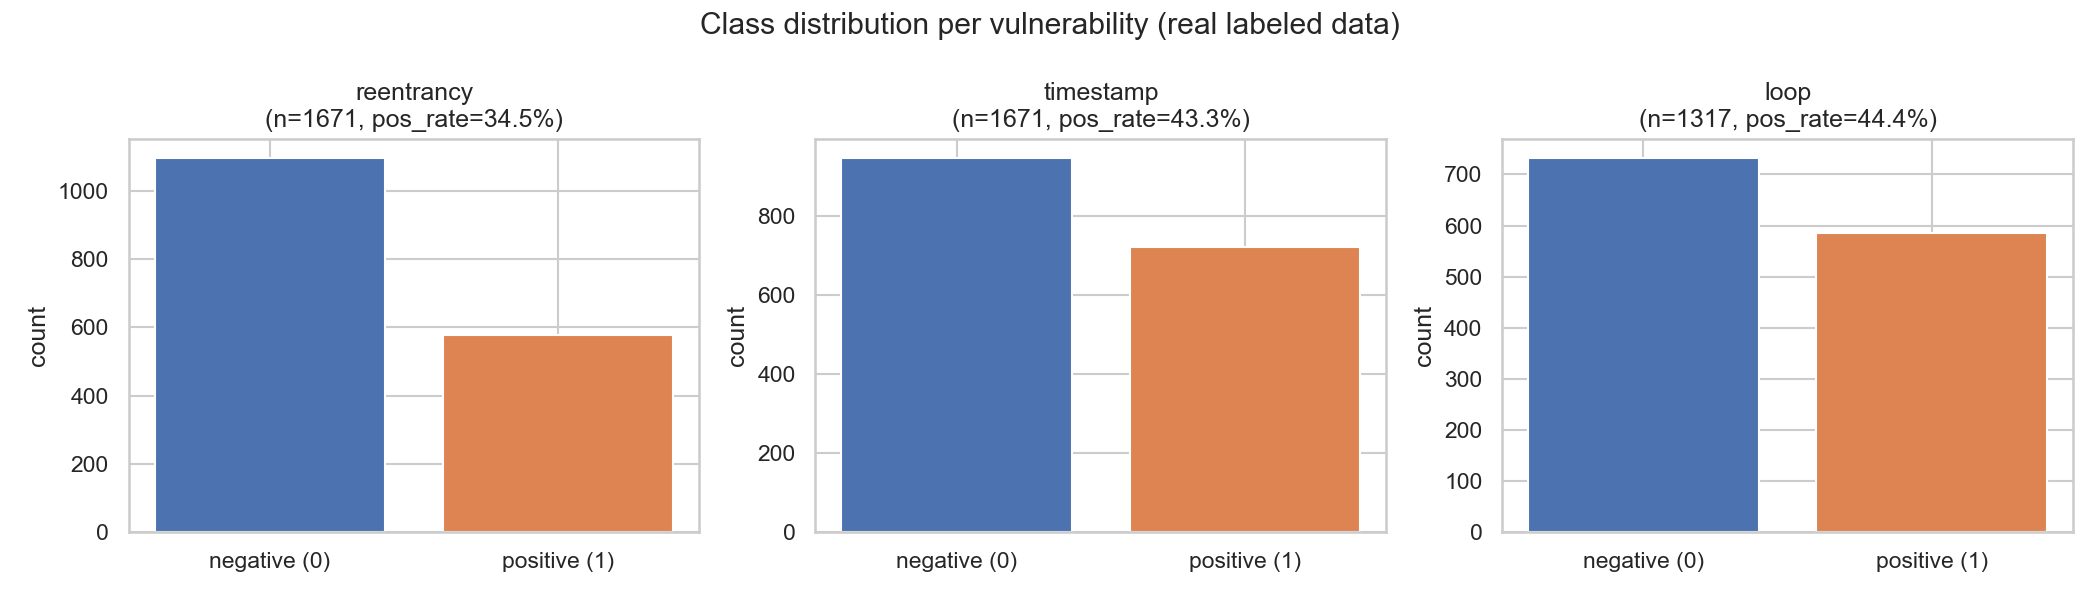
\includegraphics[width=0.95\linewidth]{class_distribution.png}
  \caption{Class distribution per vulnerability type.}
  \label{fig:class_dist}
   \end{figure}

Figure~\ref{fig:graph_size} shows the distribution of the number of core nodes per function graph, after the core-node normalization step, for each vulnerability type. Most functions are represented by a small number of core nodes, consistent with the vulnerability-focused (rather than whole-function) nature of the semantic graph representation.

\begin{figure}[H]
  \centering
  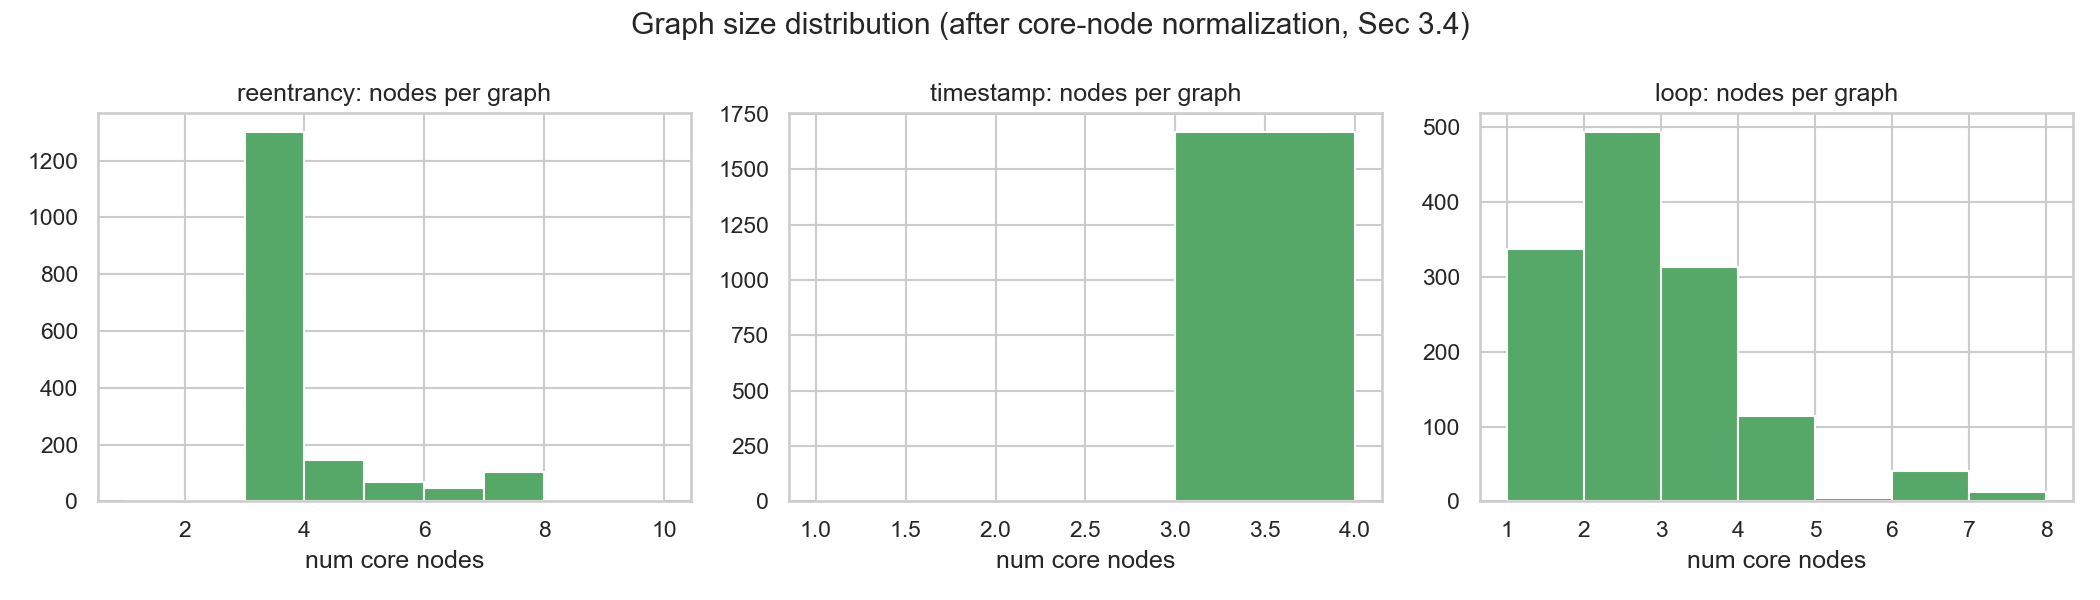
\includegraphics[width=0.95\linewidth]{graph_size_distribution.png}
  \caption{Distribution of the number of core nodes per function graph.}
  \label{fig:graph_size}
   \end{figure}

\subsection{Overall Model Comparison}

Table~\ref{tab:results_reentrancy}, Table~\ref{tab:results_timestamp}, and Table~\ref{tab:results_loop} report accuracy, precision, recall, F1-score, and ROC-AUC for all nine models on the reentrancy, timestamp, and infinite-loop datasets, respectively.

\begin{table}[htbp]
\centering
\caption{Model comparison on the reentrancy dataset}
\label{tab:results_reentrancy}
\begin{tabular}{|l|c|c|c|c|c|}
\hline
\textbf{Model} & \textbf{Acc. (\%)} & \textbf{Prec. (\%)} & \textbf{Rec. (\%)} & \textbf{F1 (\%)} & \textbf{AUC (\%)} \\ \hline
GMVD (full)     & 58.14 & 68.42 & 30.23 & 41.94 & 56.90 \\ \hline
GAT-Attention   & 53.49 & 55.17 & 37.21 & 44.44 & 49.59 \\ \hline
GNN-Mamba       & 62.79 & 76.19 & 37.21 & 50.00 & 52.73 \\ \hline
GNN-Attention   & 59.30 & 72.22 & 30.23 & 42.62 & 57.38 \\ \hline
AME-lite        & 46.51 & 42.86 & 20.93 & 28.13 & 61.76 \\ \hline
GCN             & 88.37 & 97.14 & 79.07 & 87.18 & 93.02 \\ \hline
Vanilla-RNN     & 58.14 & 70.59 & 27.91 & 40.00 & 58.84 \\ \hline
LSTM            & 48.84 & 48.00 & 27.91 & 35.29 & 58.84 \\ \hline
GRU             & 48.84 & 48.00 & 27.91 & 35.29 & 49.97 \\ \hline
\end{tabular}
\end{table}

\begin{table}[htbp]
\centering
\caption{Model comparison on the timestamp-dependence dataset}
\label{tab:results_timestamp}
\begin{tabular}{|l|c|c|c|c|c|}
\hline
\textbf{Model} & \textbf{Acc. (\%)} & \textbf{Prec. (\%)} & \textbf{Rec. (\%)} & \textbf{F1 (\%)} & \textbf{AUC (\%)} \\ \hline
GMVD (full)     & 76.07 & 76.00 & 83.52 & 79.58 & 82.42 \\ \hline
GAT-Attention   & 82.21 & 90.79 & 75.82 & 82.63 & 88.37 \\ \hline
GNN-Mamba       & 23.93 & 18.87 & 10.99 & 13.89 & 33.36 \\ \hline
GNN-Attention   & 76.07 & 72.41 & 92.31 & 81.16 & 55.34 \\ \hline
AME-lite        & 84.05 & 91.14 & 79.12 & 84.71 & 89.87 \\ \hline
GCN             & 90.80 & 88.00 & 96.70 & 92.15 & 95.67 \\ \hline
Vanilla-RNN     & 41.10 & 36.84 & 7.69  & 12.73 & 64.68 \\ \hline
LSTM            & 37.42 & 38.78 & 20.88 & 27.14 & 38.45 \\ \hline
GRU             & 33.74 & 30.23 & 14.29 & 19.40 & 36.68 \\ \hline
\end{tabular}
\end{table}

\begin{table}[htbp]
\centering
\caption{Model comparison on the infinite-loop dataset}
\label{tab:results_loop}
\begin{tabular}{|l|c|c|c|c|c|}
\hline
\textbf{Model} & \textbf{Acc. (\%)} & \textbf{Prec. (\%)} & \textbf{Rec. (\%)} & \textbf{F1 (\%)} & \textbf{AUC (\%)} \\ \hline
GMVD (full)     & 60.25 & 53.66 & 63.46 & 58.15 & 66.69 \\ \hline
GAT-Attention   & 66.53 & 61.54 & 61.54 & 61.54 & 68.72 \\ \hline
GNN-Mamba       & 64.02 & 58.18 & 61.54 & 59.81 & 71.16 \\ \hline
GNN-Attention   & 65.27 & 58.54 & 69.23 & 63.44 & 69.09 \\ \hline
AME-lite        & 64.85 & 60.00 & 57.69 & 58.82 & 69.38 \\ \hline
GCN             & 68.62 & 67.06 & 54.81 & 60.32 & 69.76 \\ \hline
Vanilla-RNN     & 65.27 & 58.97 & 66.35 & 62.44 & 68.94 \\ \hline
LSTM            & 69.04 & 67.86 & 54.81 & 60.64 & 69.06 \\ \hline
GRU             & 63.60 & 56.80 & 68.27 & 62.01 & 69.06 \\ \hline
\end{tabular}
\end{table}

Figure~\ref{fig:f1_by_model} presents the F1-score of all nine models side by side for each vulnerability type, making the relative ranking of models easier to compare visually.

\begin{figure}[H]
  \centering
  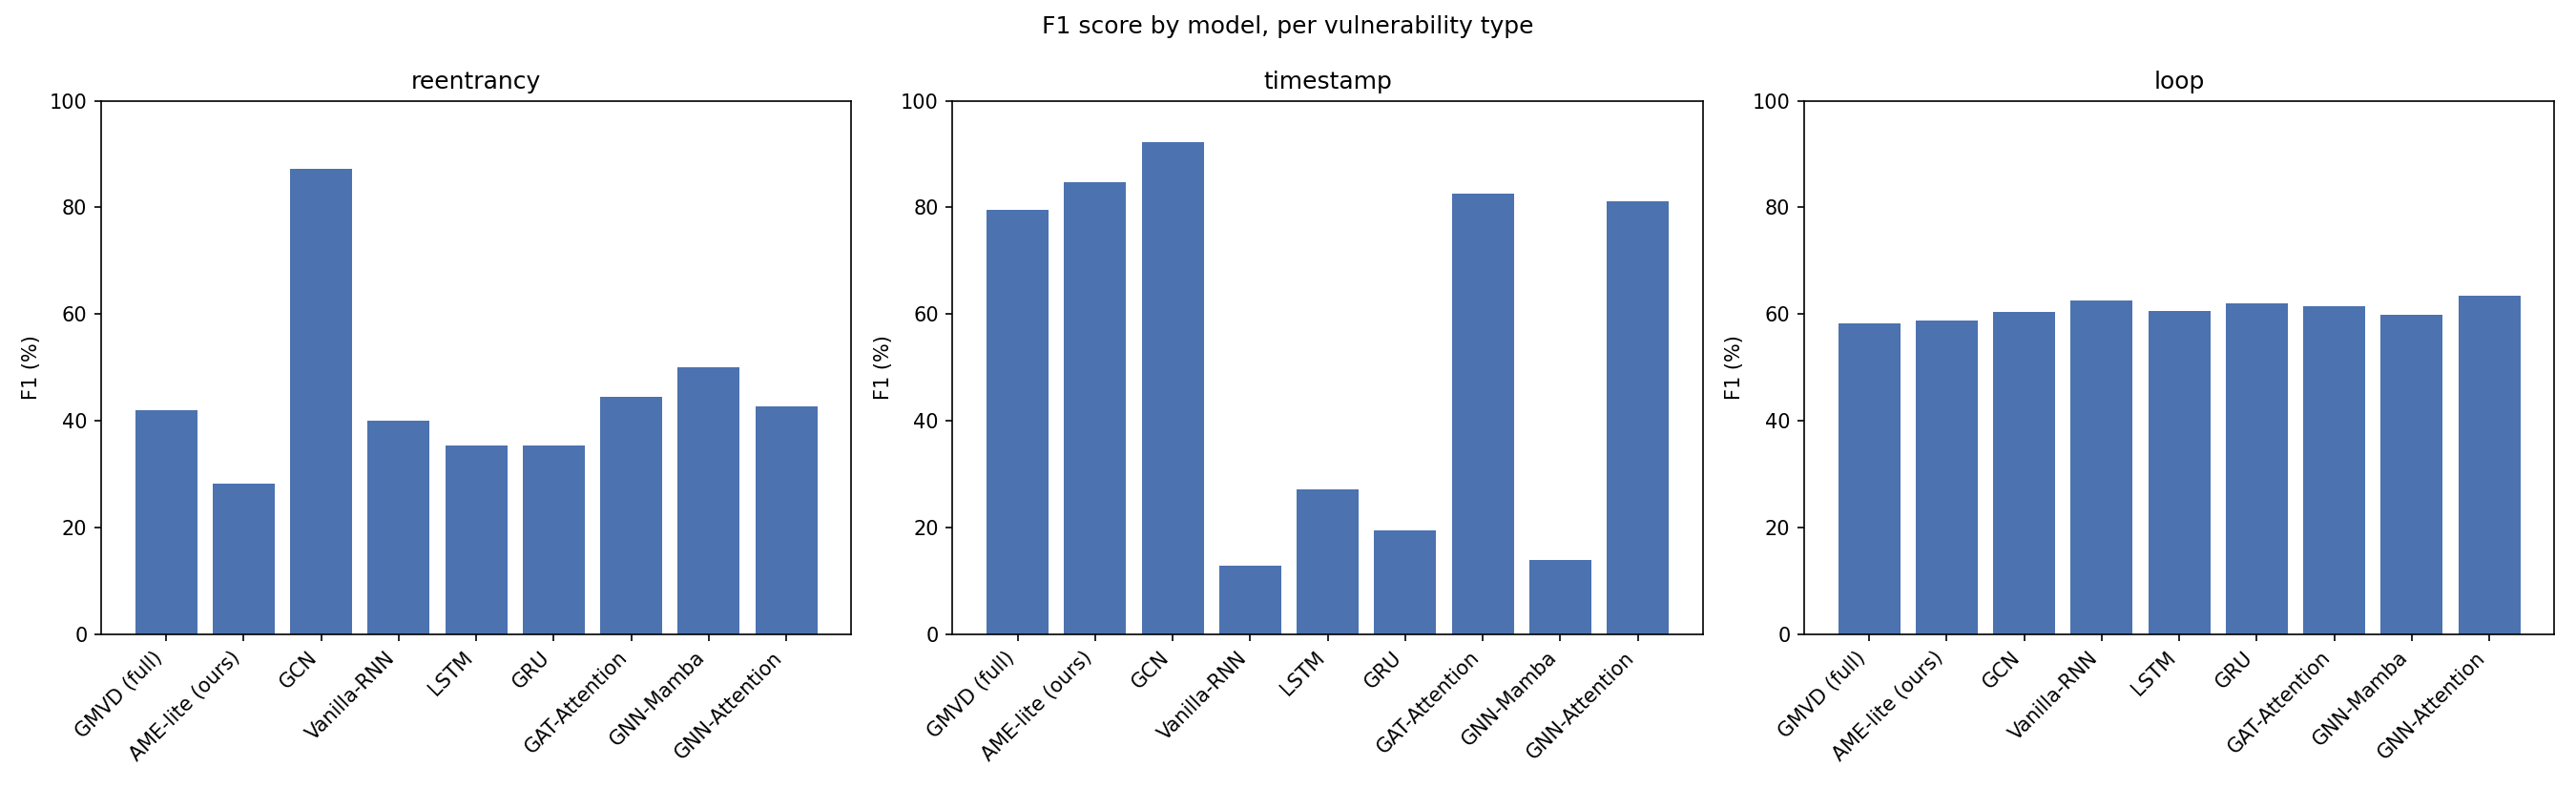
\includegraphics[width=0.98\linewidth]{f1_by_model.png}
  \caption{F1-score comparison across all trained models, per vulnerability type.}
  \label{fig:f1_by_model}
   \end{figure}

For reentrancy, the highest F1-score is achieved by the graph-only GCN baseline (87.18\%), followed by GNN-Mamba (50.00\%); GMVD (full) reaches an F1-score of 41.94\%. For timestamp dependence, GCN again achieves the highest F1-score (92.15\%), with AME-lite (84.71\%), GAT-Attention (82.63\%), and GMVD (full) (79.58\%) close behind. For infinite loop, the best F1-score is obtained by GNN-Attention (63.44\%), with GMVD (full) at 58.15\%. Across all three vulnerability types, the sequence-only baselines (Vanilla-RNN, LSTM, GRU), which have access only to the local expert patterns and not the graph structure, generally achieve lower F1-scores than the graph-based models, indicating that the semantic graph representation carries useful information beyond what the three local patterns alone provide.

\subsection{Ablation Study}

Figure~\ref{fig:ablation} isolates the four GMVD-family models -- GNN-Attention, GAT-Attention, GNN-Mamba, and GMVD (full) -- to examine the individual and combined effect of the GAT encoder and the Mamba fusion block.

\begin{figure}[H]
  \centering
  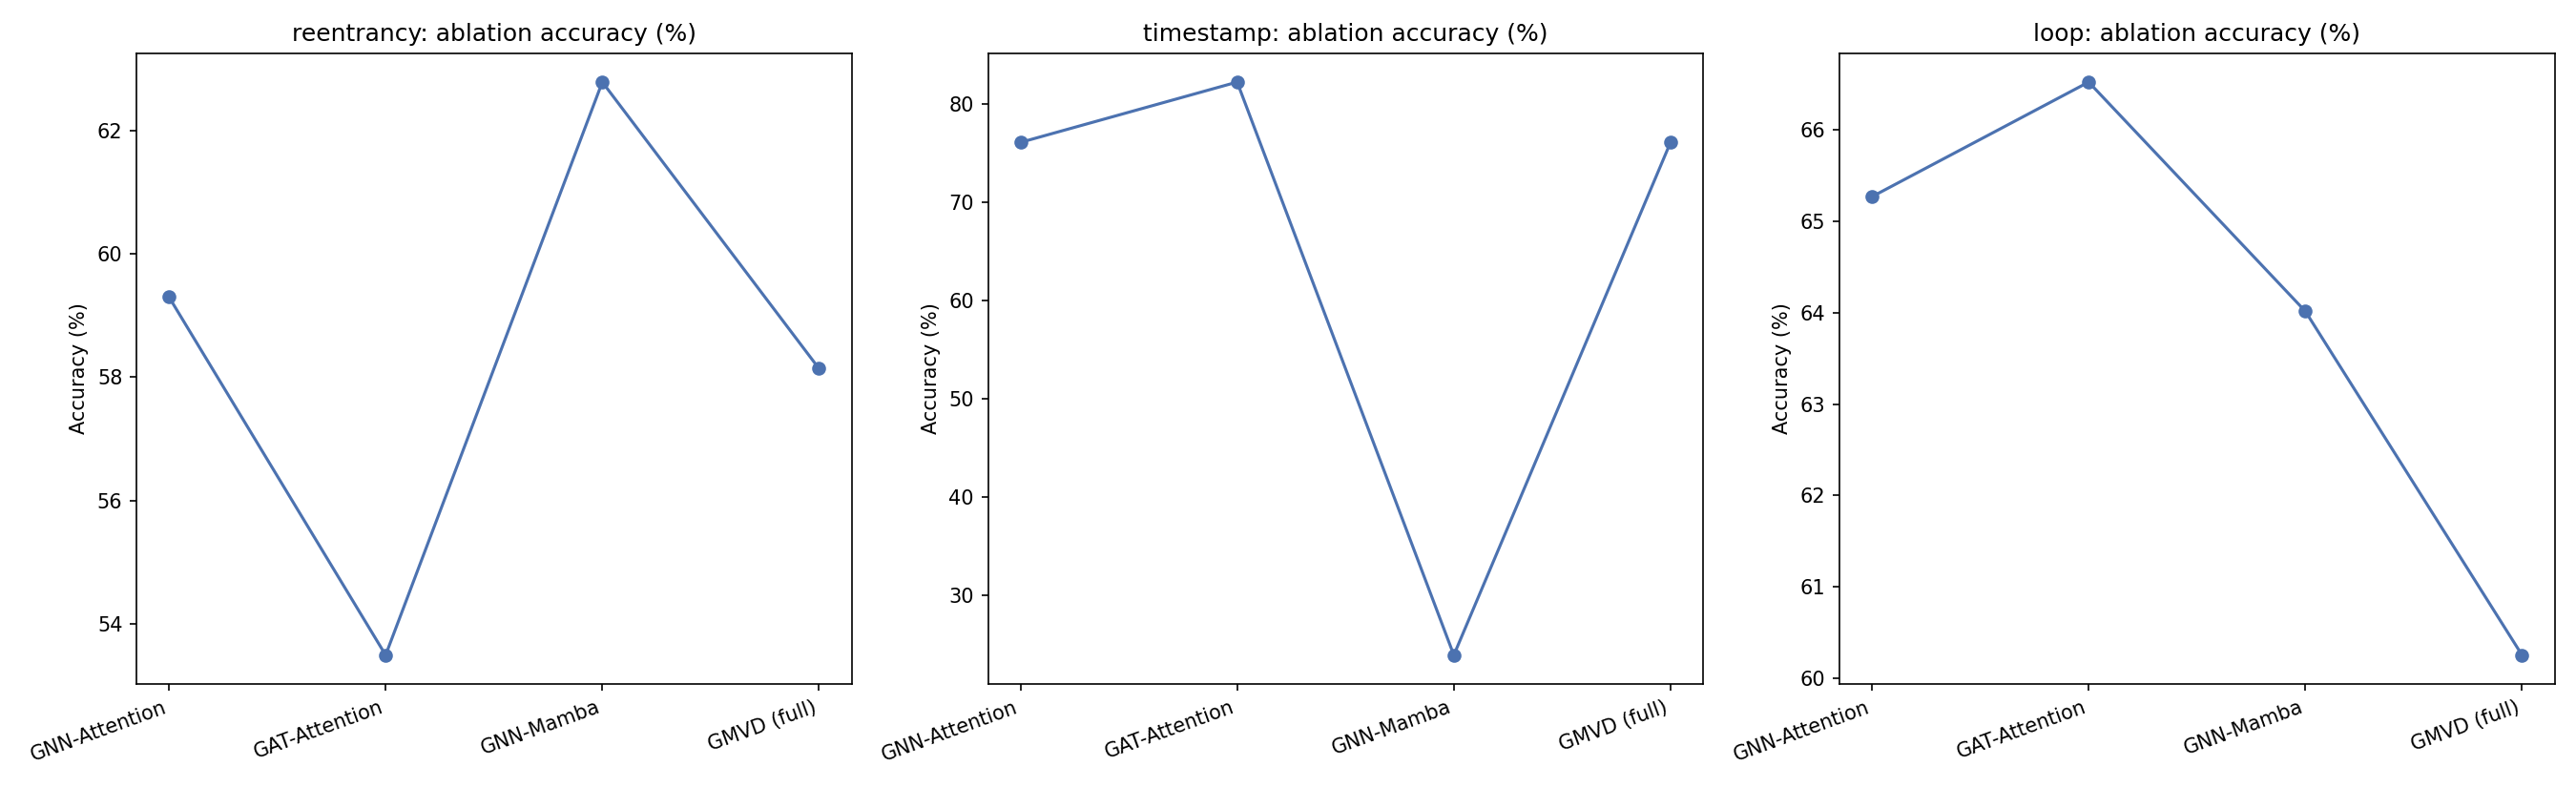
\includegraphics[width=0.98\linewidth]{ablation_study.png}
  \caption{Ablation study: accuracy of GMVD and its ablated variants, per vulnerability type.}
  \label{fig:ablation}
   \end{figure}

For reentrancy and infinite loop, adding the Mamba fusion block on top of the GAT encoder (GMVD full vs. GAT-Attention) does not increase accuracy in this experimental setting, while for timestamp dependence the picture is mixed across the four variants, with GNN-Mamba in particular showing markedly lower accuracy than the other three variants on this dataset. This suggests that the relative benefit of each architectural component (attention-based graph encoding versus selective state-space fusion) is dependent on the vulnerability type and the characteristics of its dataset, rather than uniformly additive across all three tasks.

\subsection{Confusion Matrices}

Figure~\ref{fig:confusion} shows the confusion matrices produced by GMVD (full) on the validation set for each vulnerability type.

\begin{figure}[H]
  \centering
  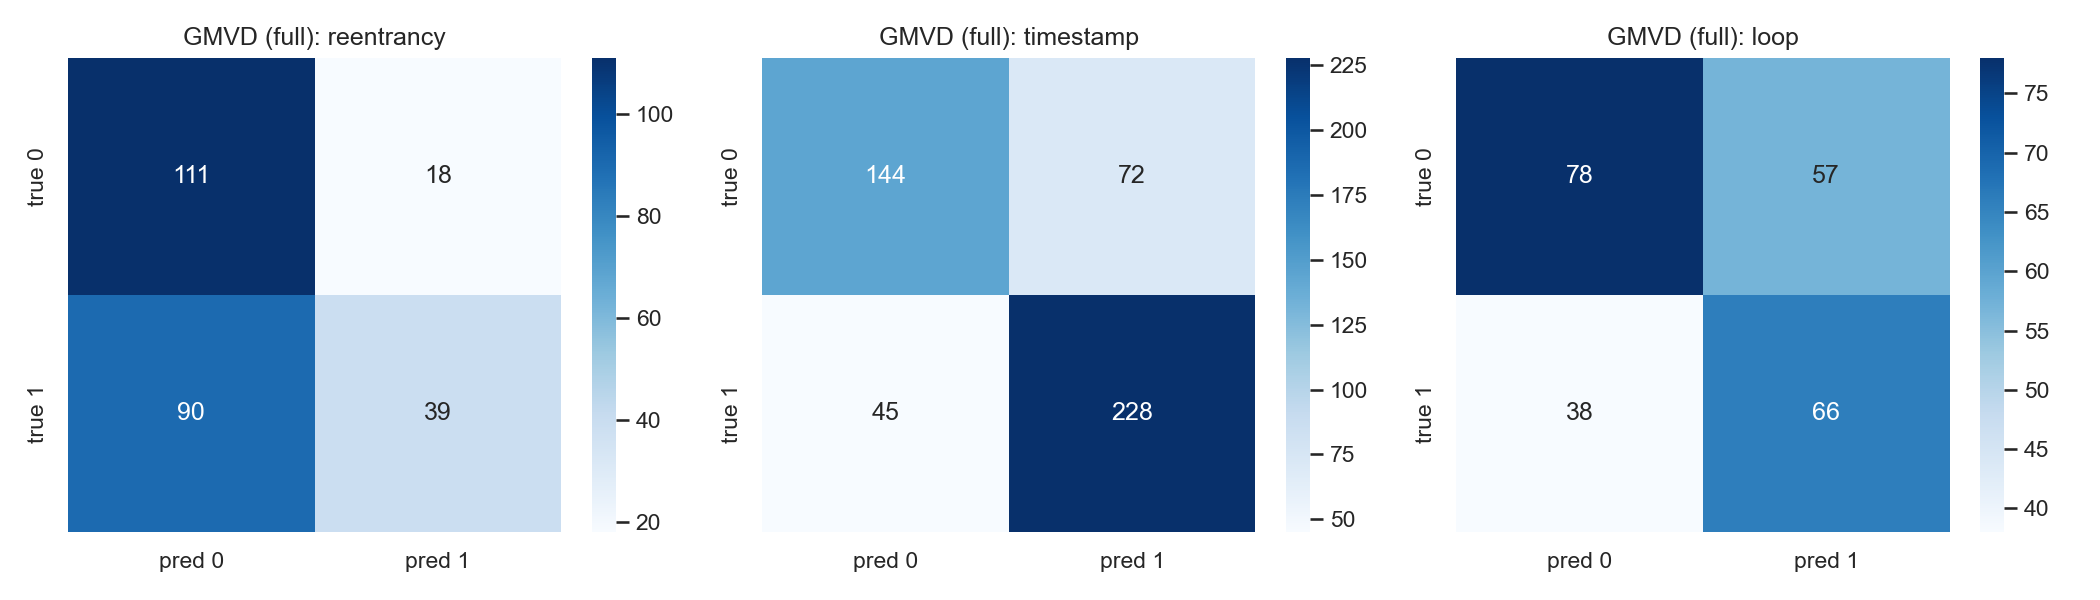
\includegraphics[width=0.98\linewidth]{confusion_matrices_gmvd.png}
  \caption{Confusion matrices of GMVD (full) on each vulnerability type.}
  \label{fig:confusion}
   \end{figure}

For reentrancy, GMVD correctly identifies 111 of 129 negative functions but only 39 of 129 positive functions, indicating a bias towards predicting the negative class at the chosen decision threshold. For timestamp dependence, the model correctly identifies 228 of 273 positive functions and 144 of 216 negative functions, giving a more balanced trade-off. For infinite loop, 78 of 135 negative and 66 of 104 positive functions are correctly classified.

\subsection{ROC Curves}

Figure~\ref{fig:roc} shows the ROC curve of GMVD (full) for each vulnerability type, together with the corresponding AUC value.

\begin{figure}[H]
  \centering
  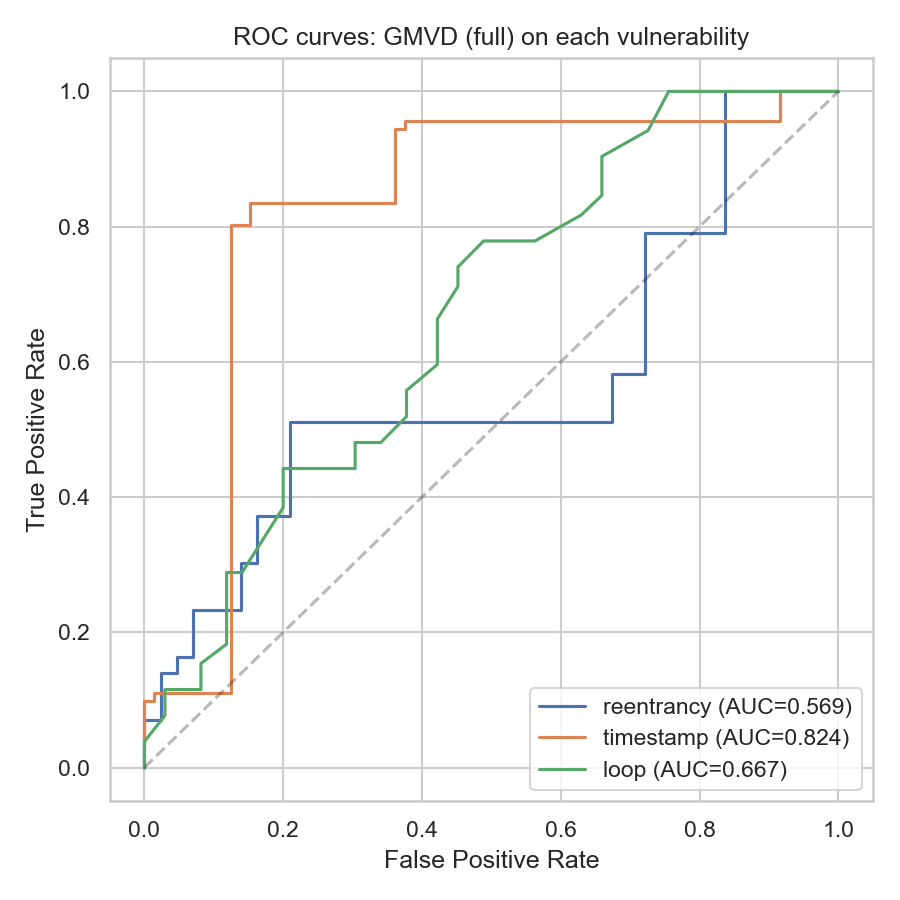
\includegraphics[width=0.7\linewidth]{roc_curves_gmvd.png}
  \caption{ROC curves of GMVD (full) on each vulnerability type.}
  \label{fig:roc}
   \end{figure}

GMVD achieves its highest ranking performance on timestamp dependence (AUC = 0.824), followed by infinite loop (AUC = 0.667) and reentrancy (AUC = 0.569), indicating that the learned probability scores are most reliably ordered for the timestamp-dependence task among the three.

\subsection{Interpretability Analysis}

A key property of GMVD is that, for every prediction, it produces an interpretability weight for each of the three local patterns and the global graph feature (Eq.~\ref{eq:interpretability}), indicating how much each contributed to the prediction. Figure~\ref{fig:interpretability} summarizes these weights over the validation set for each vulnerability type, showing (a) the percentage of examples in which each feature's weight exceeds a threshold of 0.25, and (b) the percentage of examples in which each feature receives the single largest weight.

\begin{figure}[H]
  \centering
  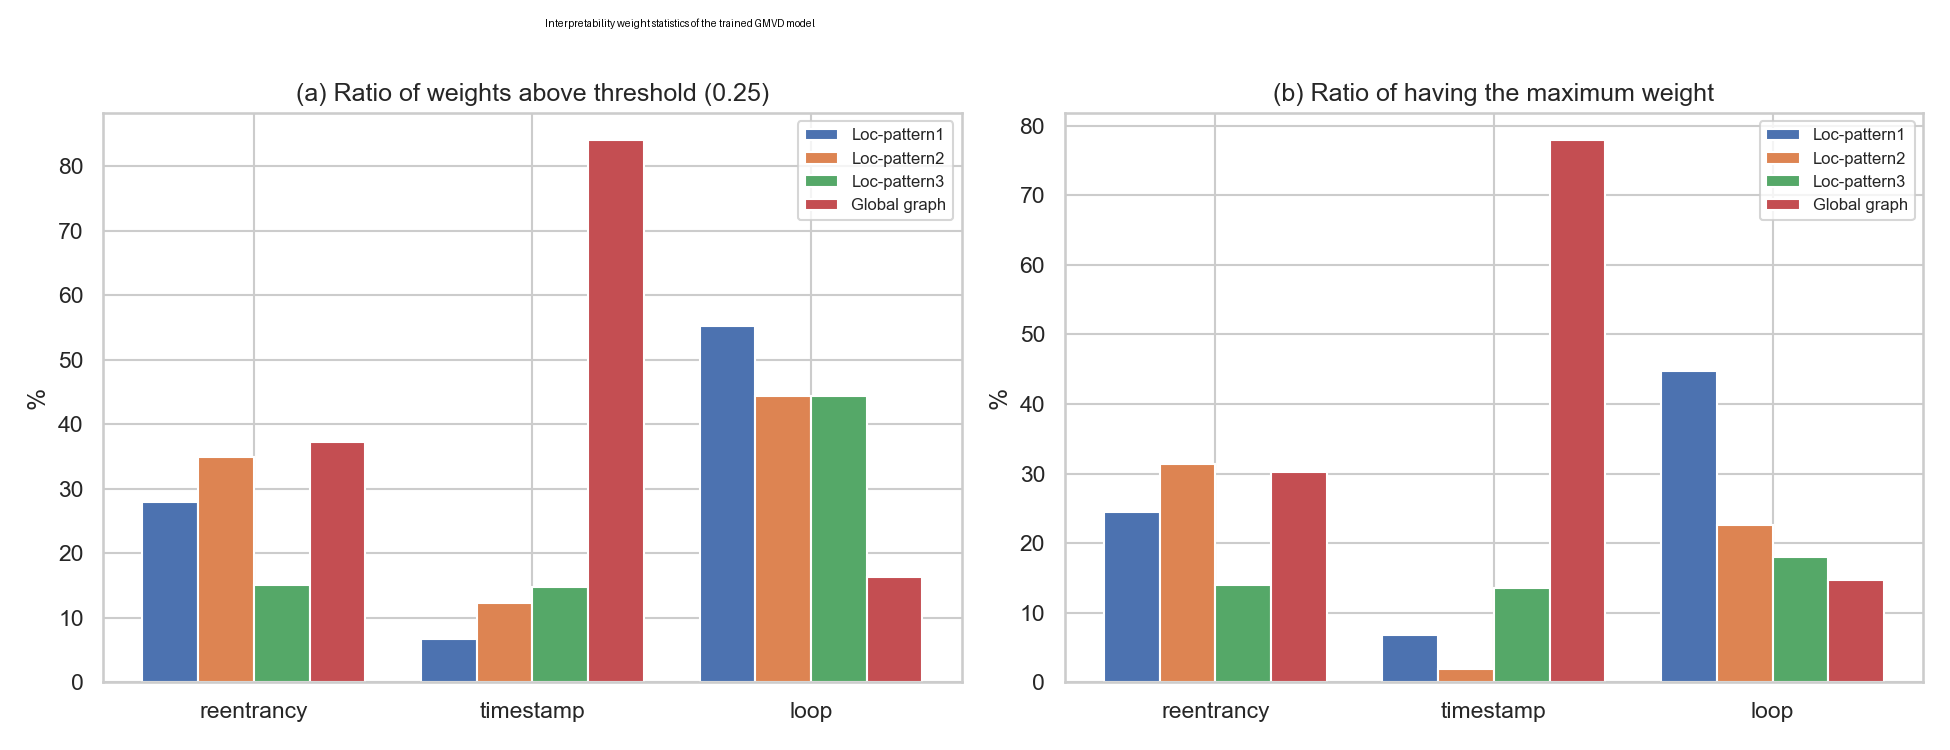
\includegraphics[width=0.98\linewidth]{interpretability_weights.png}
  \caption{Interpretability weight statistics of the trained GMVD model, per vulnerability type.}
  \label{fig:interpretability}
   \end{figure}

For reentrancy and timestamp dependence, the global graph feature $g$ most frequently receives the largest weight (30.2\% and 77.8\% of examples respectively), indicating that GMVD relies primarily on the structural (graph) representation of the function for these two vulnerability types. For infinite loop, the first local pattern $P_1$ most frequently receives the largest weight (44.7\% of examples), suggesting that for this vulnerability type the model relies more heavily on the corresponding hand-designed local pattern than on the global graph structure. This is consistent with the intuition that an infinite-loop condition is often localized to a specific loop construct that a well-designed local pattern can capture directly, whereas reentrancy and timestamp-dependence vulnerabilities can depend on relationships between statements that are better captured by the broader function graph.

\subsection{Computational Cost}

Table~\ref{tab:runtime} reports the wall-clock training time (in seconds, on the CPU-only environment described in Section~4.1.1) for GMVD (full) and the GCN baseline, on each vulnerability dataset.

\begin{table}[htbp]
\centering
\caption{Training time comparison (CPU-only)}
\label{tab:runtime}
\begin{tabular}{|l|c|c|}
\hline
\textbf{Vulnerability} & \textbf{GMVD (full) (s)} & \textbf{GCN (s)} \\ \hline
Reentrancy & 20.03 & 3.96 \\ \hline
Timestamp  & 13.09 & 5.08 \\ \hline
Infinite loop & 62.43 & 5.99 \\ \hline
\end{tabular}
\end{table}

As expected, GMVD (full) takes noticeably longer to train than the plain GCN baseline on every vulnerability dataset, reflecting the added computational cost of the GAT encoder's multi-head attention, the Mamba block's sequential state-space recurrence, and the cross-attention fusion layer, all of which the GCN baseline omits.

\subsection{Discussion}

Taken together, the results show that GMVD is able to learn a working detector for all three vulnerability types directly from labeled data, without any manually written detection rules, and additionally exposes an interpretable breakdown of its prediction in terms of the local expert patterns and the global graph feature. The interpretability analysis in particular shows that this breakdown is not uniform across vulnerability types: the model leans on the global graph structure for reentrancy and timestamp dependence, and on a local pattern for infinite loop, which is consistent with the differing nature of these three vulnerability classes. The ablation study further shows that the relative contribution of the GAT encoder and the Mamba fusion block to the model's accuracy varies by vulnerability type, indicating that neither component is uniformly necessary or sufficient on its own, and that their combination in GMVD is best understood on a per-vulnerability basis rather than as a single universal improvement.

\section{Summary}
This chapter described the software environment, the three vulnerability datasets and their statistics, the content-based train/validation splitting procedure, and the model hyperparameters used for all experiments, followed by the full experimental results: the overall comparison across all nine trained models, the ablation study, confusion matrices, ROC curves, the interpretability analysis, and a comparison of computational cost. The next chapter concludes the project and discusses directions for future work.


\chapter{Conclusions and Future Work}
\label{conclusion}
\begin{justifying}

In this project, the GMVD framework for function-level smart contract vulnerability detection was implemented end-to-end and evaluated on three vulnerability types: reentrancy, timestamp dependence, and infinite loop. The framework combines local expert pattern extraction, a Graph Attention Network encoder over a function's semantic graph, a Mamba-style selective state-space block for fusing the local patterns with the graph feature, and a cross-attention classification head that additionally produces an interpretable weight for each of the four fused features. Three ablated variants and five baseline models were implemented and trained under an identical protocol to allow a controlled comparison, giving a total of 27 trained models across the three vulnerability types.

The experimental evaluation showed that GMVD successfully learns to detect all three vulnerability types from labeled data, and that its interpretability weights provide a meaningful, vulnerability-dependent breakdown of how much the prediction relies on each local pattern versus the global graph feature -- notably, relying predominantly on the graph feature for reentrancy and timestamp dependence, and more on a local pattern for infinite loop. The ablation study showed that the relative benefit of the GAT encoder and the Mamba fusion block is not uniform across vulnerability types, indicating that the optimal architectural configuration may itself be vulnerability-dependent.

Future work will focus on extending the framework to additional vulnerability types beyond the three studied here, incorporating larger and more diverse labeled contract datasets, exploring alternative graph encoders and state-space fusion configurations, and investigating how the framework's interpretability weights could be surfaced directly to auditors as part of a practical smart-contract auditing tool.

\end{justifying}




% \bibliographystyle{agsm}
% \bibliography{references.bib}
\newpage

\begin{thebibliography}{9}
\bibitem{1}
Liu, M. and Zhang, C. ``GMVD: Smart Contract Vulnerability Detection Based on GAT-Mamba Framework.'' \emph{Research Square preprint}, DOI: 10.21203/rs.3.rs-8968309/v1, 2026.

\bibitem{2}
Liu, Z., Qian, P., Wang, X., Zhu, L., He, Q., and Ji, S. ``Smart Contract Vulnerability Detection: From Pure Neural Network to Interpretable Graph Feature and Expert Pattern Fusion.'' \emph{Proceedings of the 30th International Joint Conference on Artificial Intelligence (IJCAI)}, 2021.

\bibitem{3}
Zhuang, Y., Liu, Z., Qian, P., Liu, Q., Wang, X., and He, Q. ``Smart Contract Vulnerability Detection using Graph Neural Network.'' \emph{Proceedings of the 29th International Joint Conference on Artificial Intelligence (IJCAI)}, pp. 3283--3290, 2020.

\bibitem{4}
Velickovic, P., Cucurull, G., Casanova, A., Romero, A., Lio, P., and Bengio, Y. ``Graph Attention Networks.'' \emph{International Conference on Learning Representations (ICLR)}, 2018.

\bibitem{5}
Gu, A. and Dao, T. ``Mamba: Linear-Time Sequence Modeling with Selective State Spaces.'' \emph{arXiv preprint arXiv:2312.00752}, 2023.

\end{thebibliography}

\clearpage
\appendix
\chapter{BIO-DATA}
\null
\null
\null
\null

\begin{table}[H]
\centering

\begin{tabular}{cl}
\toprule
\textbf{Name:}          &   AMEESHA PATEL                                                                                                                    \\ \midrule
\textbf{Address:}       & \begin{tabular}[c]{@{}l@{}}[Your Address Line 1],\\ {[}City{]},\\{[}District, State - PIN{]}\end{tabular}                             \\ \midrule
\textbf{Email:}         &  vatsal193218@gmail.com                   \\ \midrule
\textbf{Contact No.:}   & [Your Contact Number]                                                                                                                               \\ \midrule
\textbf{Qualification:} & \begin{tabular}[c]{@{}l@{}}M.Tech in Information Technology , \\National Institute of Technology Karnataka Surathkal  \\ \\B.Tech in [Your Branch], \\{[}Your B.Tech Institution{]},\end{tabular} \\ \bottomrule
\end{tabular}
\end{table}
\null
\null


\end{document}
